
%(BEGIN_QUESTION)
% Copyright 2010, Tony R. Kuphaldt, released under the Creative Commons Attribution License (v 1.0)
% This means you may do almost anything with this work of mine, so long as you give me proper credit

Denne strømningsmåleren (Annubar-strømningselement, Yokogawa DP-transmitter) brukes til å måle luftstrøm gjennom et stort rør. Installasjonen kan imidlertid forbedres:

$$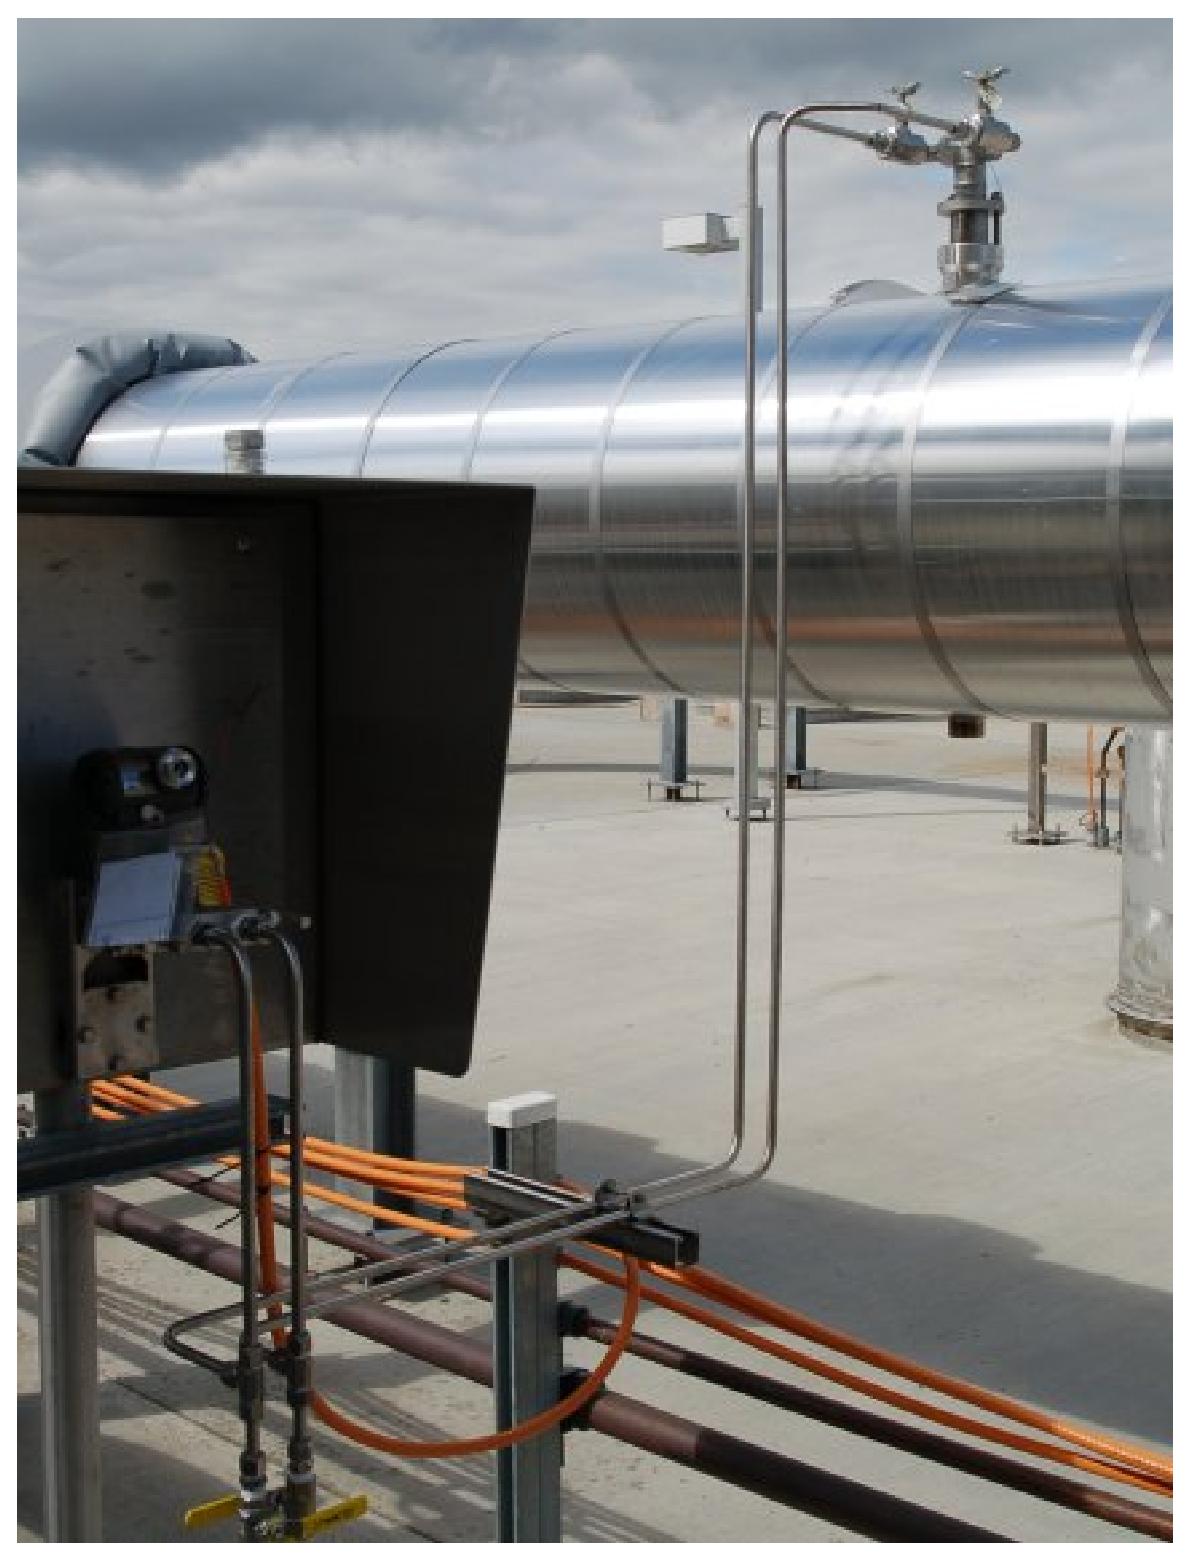
\includegraphics[width=15.5cm]{i01400x01.eps}$$

Forklar hvordan du ville forbedret denne strømningsmålerinstallasjonen dersom du fikk i oppdrag å bygge den om.

\underbar{file i01400}
%(END_QUESTION)





%(BEGIN_ANSWER)

Siden dette er en luftprosess (gass), bør DP-transmitteren monteres {\it over} strømningselementet, ikke under. Slik den er bygget nå, må en tekniker jevnlig åpne utluftingsventilene (plassert i de nederste ``tee''-koblingene på impulsrørene) for å tappe ut eventuell oppsamlet væske.

%(END_ANSWER)





%(BEGIN_NOTES)

{\bf Dette spørsmålet er ment for eksamen og ikke arbeidsark!}.

%(END_NOTES)

